\documentclass{LMUexercise}
%
%
\usepackage[utf8]{inputenc}
\usepackage{paralist}
%
\begin{document}
%
%\ExSheet{}{}{}
%{}
%
%
\vspace*{1cm}
\begin{center}
\textbf{\Large ObsPy Workshop at SED, Zürich 09/2012\\ --\\ ObsPy Practical}
\end{center}
\vspace*{1.2em}
%
% -----------------------------------------------------------------------------
%
This practical intends to demonstrate how ObsPy can be used to develop
workflows for data processing and analysis that have a short, easy to read and
extensible source code. The overall task is to automatically estimate local
magnitudes of earthquakes using data of the SED network. We will start with
simple programs with manually specified, hard-coded values and build on them
step by step to make the program more flexible and dynamic.\\
Some details in the magnitude estimation should be done a little bit different
technically but we rather want to focus on the general workflow here.\\
For help with all problems try to find informations in the ObsPy online
documentation at \verb#http://docs.obspy.org# (e.g. use the search) and the
Tutorial at \verb#http://tutorial.obspy.org#.\\ In addition, all solutions are
available in the subfolder of the same name.
\vspace*{1em}

\begin{center}
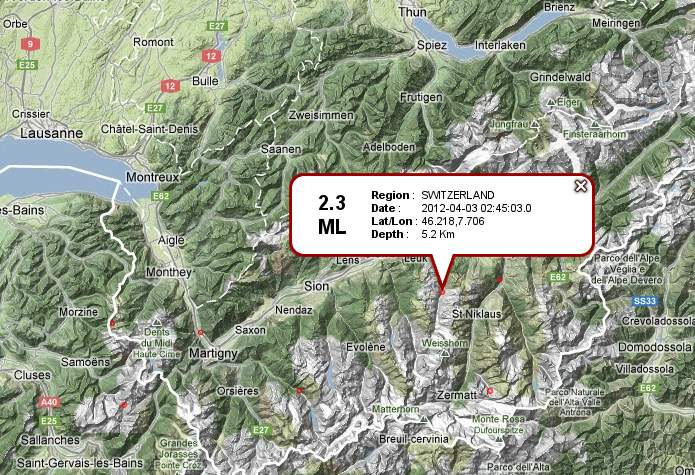
\includegraphics[width=0.63\textwidth]{data/event.jpg}\\
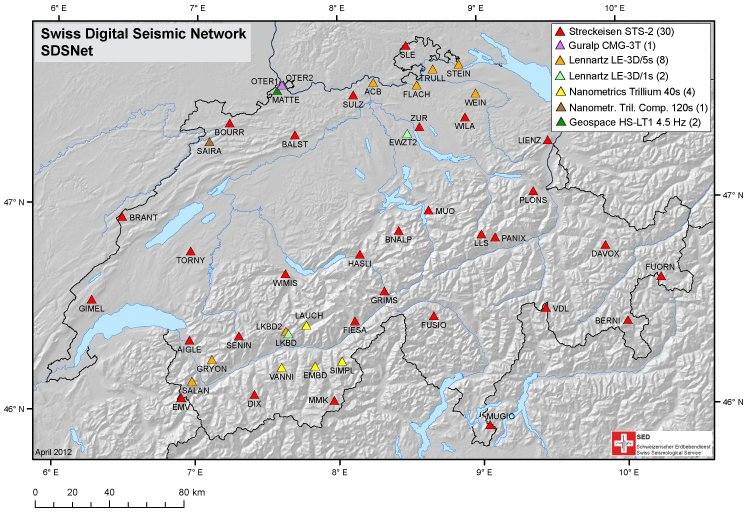
\includegraphics[width=0.69\textwidth]{data/network_map.jpg}
\end{center}
\vspace*{1em}
\clearpage


\exercise{Request Earthquake Information from EMSC/NERIES/NERA}\\
%\begin{itemize}[(a)]
%\item
Fetch a list of events from EMSC for the region of Valais/SW-Switzerland on 3rd April
of 2012. Use the \verb#Client# provided in \verb#obspy.neries#. Note down the
catalog origin times, epicenters and magnitudes.
%\end{itemize}
\vspace*{2.5em}

\exercise{Estimate Local Magnitude}\\
\begin{enumerate}[a)]
\item
Use the file \verb#LKBD_WA_CUT.MSEED# to read \verb#MiniSEED# waveform data of
the larger earthquake. These data have already been simulated to (demeaned)
displacement on a Wood-Anderson seismometer (in meter) and trimmed to the right
time span. Compute the absolute maximum for both N and E component and use the
larger value as the zero-to-peak amplitude estimate. Estimate the local
magnitude $M_{lh}$ used at SED using a epicentral distance of $d_{epi}=20$
(km), $a=0.018$ and $b=2.17$ with the following formula (mathematical functions
are available in the \verb#math# module):

\[
M_{lh} = \log_{10}\left(amp * 1000\mathrm{\frac{mm}{m}}\right) + a * d_{epi} + b
\]
\item
Calculate the epicentral distance from the station coordinates
(46.387$^\circ$N, 7.627$^\circ$E) and catalog epicenter fetched above
(46.218$^\circ$N, 7.706$^\circ$E). Some useful routines for such tasks are
included in \verb#obspy.core.util.geodetics#.
\end{enumerate}
\vspace*{3.0em}

\exercise{Seismometer Correction/Simulation}\\
\begin{enumerate}[a)]
\item
Modify the existing code and use the file \verb#LKBD.MSEED# to read the
original \verb#MiniSEED# waveform data in counts. Set up two dictionaries
containing the response information of both the original instrument (a
\verb#LE3D-5S#) and the Wood-Anderson seismometer in poles-and-zeros
formulation. Please note that for historic reasons the naming of keys differs
from the usual naming.  Each \verb#PAZ# dictionary needs to
contain \verb#sensitivity# (overall sensitivity of seismometer/digitizer
combination), \verb#gain# (A0 / normalization factor), \verb#poles# and
\verb#zeros#. Check that the value of \verb#water_level# is not too high, to
avoid overamplified low frequency noise at short-period stations. After the
instrument simulation, trim the waveform to a shorter time window around the
origin time (\verb#2012-04-03T02:45:03#) and calculate $M_{lh}$ like before.
Use the following values for the \verb#PAZ# dictionaries:
{\footnotesize
\begin{verbatim}
    LE3D-5S  'gain': 1.009
             'poles': [-0.885+0.887j,
                       -0.885-0.887j,
                       -0.427+0j]
             'sensitivity': 167364000.0
             'zeros': [0j, 0j, 0j]

    Wood-Anderson  'gain': 1
                   'sensitivity': 2800
                   'poles': [-6.2832-4.7124j, -6.2832+4.7124j]
                   'zeros': [0j]
\end{verbatim}
}
\item
Instead of the hard-coded values, read the response information from a locally
stored \verb#dataless SEED# (\verb#LKBD.dataless#). Use the \verb#Parser# of
module \verb#obspy.xseed# to extract the poles-and-zeros information of the
used channel.
\item
We can also request the response information from WebDC using the ArcLink
protocol. Use the \verb#Client# provided in \verb#obspy.arclink# module
(specify \verb#user="sed-workshop@obspy.org"#).
\end{enumerate}
\vspace*{1.5em}

\exercise{Fetch Waveform Data from WebDC}\\
\begin{enumerate}[a)]
\item
Modify the existing code and fetch waveform data around the origin time given above
for station \verb#LKBD# (network \verb#CH#) via ArcLink from WebDC using
\verb#obspy.arclink#. Use a wildcarded \verb#channel="EH*"# to fetch all three
components. Use keyword argument \verb#metadata=True# to fetch response
information and station coordinates along with the waveform. The \verb#PAZ# and
coordinate information will get attached to the \verb#Stats# object of all
traces in the returned \verb#Stream# object during the waveform request
automatically. During instrument simulation use keyword argument
\verb#paz_remove='self'# to use every trace's attached \verb#PAZ# information
fetched from WebDC. Calculate $M_{lh}$ like before.
\item
Use a list of station names (e.g. \verb#LKBD#, \verb#SIMPL#, \verb#DIX#) and
perform the magnitude estimation in a loop for each station. Use a wildcarded
\verb#channel="[EH]H*"# to fetch the respective streams for both short-period
and broadband stations. Compile a list of all station magnitudes and compute
the network magnitude as its median (available in \verb#numpy# module).
\item
Extend the network magnitude estimate by using all available stations in
network \verb#CH#. Get a list of stations using the ArcLink client and loop over
this list. Use a wildcarded \verb#channel="[EH]H[ZNE]"#, check if there are
three traces in the returned stream and skip to next station otherwise
(some stations have inconsistent component
codes). Put a \verb#try/except# around the waveform request and skip to the
next station and avoid interruption of the routine in case no data can be
retrieved and an Exception gets raised. Also add an \verb#if/else# and use
$a=0.0038$ and $b=3.02$ in station magnitude calculation for epicentral
distances of more than 60 kilometers.
\end{enumerate}
\vspace*{2.5em}

\exerciseS{Fetch Waveform Data from WebDC}\\
If there is still time, in this additional advanced exercise we can enhance the routine to be independent of a-priori known origin times by using a coincidence network trigger for event detection.
\begin{itemize}
\item fetch a few hours of Z component data for 6 stations in Valais/SW-Switzerland
\item run a coincidence trigger like shown in the ObsPy Tutorial at \verb#http://tutorial.obspy.org#
\item loop over detected network triggers, store the coordinates of the closest station as the epicenter
\item loop over triggers, use the trigger time to select the time window and use the network magnitude estimation code like before
\end{itemize}
\vspace*{2.5em}


\end{document}
